\documentclass{beamer}
\usetheme[pageofpages=of,% String used between the current page and the
                         % total page count.
          bullet=circle,% Use circles instead of squares for bullets.
          titleline=true,% Show a line below the frame title.
          alternativetitlepage=true,% Use the fancy title page.
       %   titlepagelogo=logo-polito,% Logo for the first page.
       %   watermark=watermark-polito,% Watermark used in every page.
       %   watermarkheight=100px,% Height of the watermark.
       %   watermarkheightmult=4,% The watermark image is 4 times bigger
                                % than watermarkheight.
          ]{Torino}

\setbeamertemplate{footline}{
  \begin{beamercolorbox}[wd=\paperwidth,ht=1ex,dp=1ex]{footline}
    \vspace{5pt} \hspace{1em} \insertframenumber/\inserttotalframenumber
  \end{beamercolorbox}
}

\author{Brendon J. Brewer}
\title{STATS 331 -- Introduction to Bayesian Statistics}
\institute{The University of Auckland}
\date{}


\linespread{1.3}
\usepackage{minted}
\usepackage[utf8]{inputenc}
\usepackage{dsfont}
\newcommand{\given}{\,|\,}


\begin{document}

\frame{\titlepage}

\begin{frame}
\begin{center}
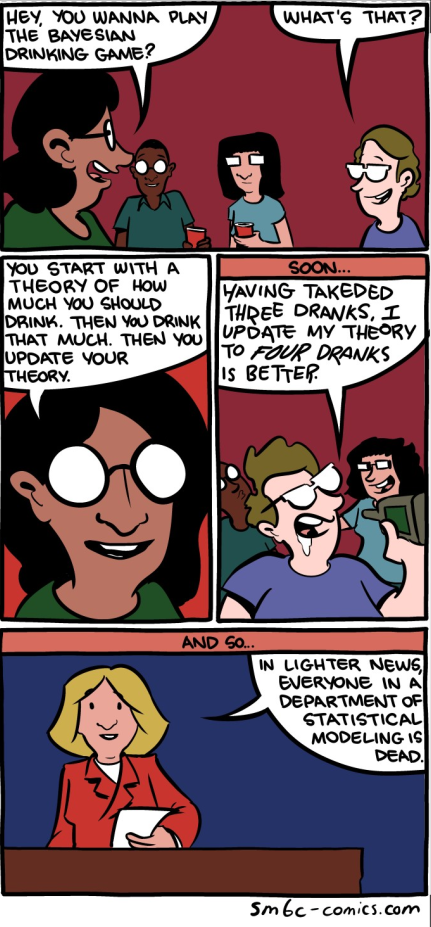
\includegraphics[width=0.3\textwidth]{images/drinking_game.png}
\end{center}

Do not attempt at home.

\end{frame}

\begin{frame}
\frametitle{Maths, Probability, and R}

\begin{itemize}
\item To understand and use Bayesian statistics, we will
require some mathematics and some R programming
skills.\pause
\item  In this lecture we will briefly review some of the concepts
that we will need.\pause
\item If you are a bit rusty, there will be plenty of opportunity to
brush up. If you are already a pro, great!
\end{itemize}

\end{frame}


\begin{frame}
\frametitle{Probability}
We will use probability extensively in this course. You may have previous
experience with it (e.g. from STATS 125), which may help. However, the way we
use it is different.



\end{frame}


\begin{frame}
\frametitle{Probability}
We will use probability extensively in this course. You may have previous
experience with it (e.g. from STATS 125), which may help. However, the way we
use it is different.



\end{frame}

\begin{frame}
\frametitle{Probability --- Product Rule --- Traditional}
If we have two {\color{red} events} $A$ and $B$, the probability that both
{\color{red} occur} is given by the product rule:

\begin{align}
P(A \cap B) &= P(A)P(B \given A)
\end{align}

The `$\cap$' means intersection, but we will not see it again.



\end{frame}

\begin{frame}
\frametitle{Probability --- Product Rule --- Bayesian}
If we have two {\color{blue} propositions} or
{\color{blue} statements}
 $A$ and $B$, the probability that both {\color{blue} are true}
is given by the product rule:

\begin{align}
P(A, B) &= P(A)P(B \given A) \\
        &= P(B)P(A \given B).
\end{align}\pause

Note the change in terminology, and the notation. The comma means `and',
and the vertical bar means `given'.



\end{frame}


\begin{frame}
\frametitle{Probability --- Bayesian}
\begin{itemize}
\item In 331 we apply probability to {\color{blue} propositions
or statements}, not events. \pause
\item Probabilities represent the fact that we don't know everything.
You can think of it as `plausibility'. \pause
\item There is not a concept of `randomness' in the
sense of variability.\pause
\item If a quantity varies (e.g., the maximum daily temperature $T$),
really there’s more than one quantity
$(T_{\rm yesterday}$, $T_{\rm today}, T_{\rm tomorrow}, ...)$. We may or may
not know their values.
\end{itemize}

\end{frame}

\begin{frame}
\frametitle{The Most General Product Rule}
The product rule also holds if every term has `given $C$' on the right hand
side, where $C$ is any third statement:

\begin{align}
P(A, B \given C) &= P(A \given C)P(B \given A, C).
\end{align}\pause

If this is a bit much at this point, don't worry --- we have ways of making it
seem easy.

\end{frame}


\begin{frame}
\frametitle{Product Rule Example}
Consider a particular individual person, who you know very little about.

\begin{itemize}
\item Suppose the probability the person is male is 50\%.
\item Suppose the probability that a male is taller than 6 feet is
30\%.
\item What is the probability that the person is both male and
taller than 6 feet?
\end{itemize}

\end{frame}

\begin{frame}
\frametitle{Product Rule Example}
By the product rule,

\begin{align}
P(\textnormal{male}, \textnormal{tall})
    &= P(\textnormal{male})P(\textnormal{tall} \given \textnormal{male})\\
    &= 0.5 \times 0.3\\
    &= 0.15.
\end{align}

\end{frame}

\begin{frame}
\frametitle{Product Rule --- Probability Interpretation}
Notice that the story was about a {\em single individual} whose properties
were {\em unknown to you}. This is Bayesian.\\[0.5em]\pause

A similar question could ask for the
{\em proportion of the population} that is male and tall.
The mathematics would be exactly the same, but the meaning of the quantities
is different.
\end{frame}


\end{document}

